
\chapter{Benchmark Development}

The main objective of this work is to provide a benchmark suite for \ac{GASPI} to evaluate the performance of implementations such as \acs{GPI}-2. First, a series of microbenchmarks are developed that measure the performance of the basic communication routines. The microbenchmarks are supplemented by application benchmarks that utilized \ac{GASPI} in an application context with common access patterns. Both benchmark types are integrated in a unified suite that provides a simple user interface with fine-grained control over the individual benchmarks. This chapter serves two purposes: First, the program usage is documented to facilitate its deployment and to discuss how the software may be extended or modified. Second, the design indents behind the program's structure and the functionality of each individual benchmark are explained.

\section{Program Usage}

To run the \ac{GBS}, a successfully compiled version of the \gpi library or another implementation of the \ac{GASPI} standard is required. The path to the compiled \gpi files need to be specified in the file \code{paths.sh} in the \code{scripts} directory. After providing the correct path, \ac{GBS} may be compiled by issuing the \code{make} command in the \ac{GBS} directory. The created binary should be placed in the subdirectory \code{build} by default.

The \ac{GBS} program  is intended to be run via the \code{gaspi\_run} command supplied with \gpi. However, if only information on the parameters or the benchmarks should be obtained, the \ac{GBS} program may be launched directly with either the \code{-h} parameter to print the program's usage or with the \code{-list} parameter to get a list of all available benchmarks. The output of the help command is shown in \autoref{lst:impl:gbs-help}.

\begin{lstlisting}[style=console,captionpos={b},caption={Description of all available program parameters.},label=lst:impl:gbs-help]
USAGE for "build/gaspi-benchmark"
###########################
-bench=VALUE[,VALUE,...,VALUE] : specify a list of benchmarks to run (optional).
-maxruns=VALUE: specify the maximal number of repetitions in one single test (Default: 1024).
-minruns=VALUE: specify the minimal number of repetitions in one single test (Default: 10).
-aggregate=VALUE: specify the number of transfers to aggregate before flush (Default: 1).
-reducethres=VALUE: specify the transfer size in bytes from which to reduce the number of repetitions. Zero disables this (Default: 65536).
-warmup=VALUE: specify the percentage of warm-up repetitions before the actual measurement (Default: 10%).
-size-start=VALUE: specify the number of bytes to transfer as the first data point (Default: 1).
-size-stop=VALUE: specify the number of bytes to transfer as the last data point (Default: 4194304).
-size-factor=VALUE: specify the factor to increase the transfer size with (Default: 2).
-grid-size-start=VALUE: Application benchmark Grid: Specify the starting size of the grid (Default: 16).
-grid-size-stop=VALUE: Application benchmark Grid: Specify the final size of the grid (Default: 2048).
-grid-size-factor=VALUE: Application benchmark Grid: Specify the factor to increase the grid size with (Default: 2).
-grid-iterations=VALUE: Application benchmark Grid: Specify the number of time steps to perform for one single measurement (Default: 128).
-grid-reducethres=VALUE: Application benchmark Grid: Specify the threshold for the grid size from which the number of measurement repetitions is reduced. Zero disables this (Default: 512).
-grid-minruns=VALUE: Application benchmark Grid: Specify the minimal number of repetitions for one grid size (Default: 10).
-grid-maxruns=VALUE: Application benchmark Grid: Specify the maximal number of repetitions for one grid size (Default: 128).
-grid-threads=VALUE: Application benchmark Grid: Specify the number of processing threads (Default: 1).
-time-combined: Fetch time measurements from all nodes and report the average instead of only the result from rank 0 (Default: false).
-test: Run benchmarks with the minimum number of repetitions or iterations.
-list: List the number of available benchmarks and exit.
-h: displays this help and exit.
###########################
\end{lstlisting}


To actually run the benchmark, the program needs to be launched either manually with the help of \code{gaspi\_run} from the \gpi library or with the \code{launch.sh} script provided with the \ac{GBS} files. Most importantly, a machine file needs to be created which contains a list of host names with nodes on which the program is spawned. The path of the machine file is also specified in \code{paths.sh}. With the help of the \code{launch.sh} script, all necessary environment variables are set up automatically on the remote nodes, requiring no additional manual configuration. In \autoref{lst:impl:gbs-launch} an example is shown how the \ac{GBS} benchmark is launched with an optional argument that limits the measurement repetitions per benchmark.

\begin{lstlisting}[style=console,captionpos={b},caption={Example launch of the \ac{GBS} program.},label=lst:impl:gbs-launch]
./launch.sh build/gaspi-benchmark -maxruns=1
\end{lstlisting}

If the program is run without any arguments, all available benchmarks will be run with a set of sensible default parameters that are shown in \autoref{lst:impl:gbs-help}. The values of the default parameters are loosely based on the \ac{IMB} and \ac{OMB} microbenchmarks. The first set of arguments given in  \autoref{lst:impl:gbs-help} is related to the series of microbenchmarks. Setting \eg \code{-maxruns=1} causes the maximum number of repetitions to be set to 1 when executing all microbenchmarks. Since application benchmarks may have their own metrics and parameters, command line arguments are not shared across different application benchmarks. For the grid benchmark, the respective parameters are explained in detail in \secref{ssec:impl:grid}.

The output format of the program is identical to the \ac{IMB} program output: The results of all executed benchmarks are concatenated and printed on the command line in a human-readable syntax. This format was chosen over a machine-compatible format like the \ac{CSV} format, because the \ac{GBS} program is meant to behave as similar as possible to the \ac{IMB} or \ac{OMB} benchmarking suites. In order to convert the output of \ac{IMB}, \ac{OMB} or \ac{GBS} to \ac{CSV} format, a separate program has been developed that is explained in \secref{sec:impl:output-conversion}.

\section{General Program Architecture}

The benchmark environment essentially consists of three files:
\begin{itemize}
	\item \code{gbs\_main.c}
	\item \code{gbs\_benchmark.c}
	\item \code{gbs\_microbenchmarks.c}
\end{itemize}

The \code{gbs\_main.c} file is the main program that calls all other functions. It sets up the \ac{GASPI} environment and delegates all other procedures such as program argument parsing and evaluation, benchmark initialization and execution and finally resource deallocation and program shutdown. The benchmarks to be executed are either retrieved from the command line or, if no benchmark list is provided, all benchmarks are run in a defined sequence. 

\subsection{Benchmark Registration and Sequencing}
\label{ssec:impl:arch:gbs-benchmark}

The program code in the file \code{gbs\_benchmark.c} is responsible for iterating through the list of benchmarks to be executed and running the respective benchmark function. Furthermore, the configuration of the current benchmark run is written to the console in a formatted fashion. All benchmark functions need to implement a common interface, \ie the respective benchmark function that is called in the \code{gbs\_benchmark.c} module must have a function signature as shown in \autoref{lst:impl:gbs-benchmark-func}. The definition of the structure in the function's argument is given in \autoref{lst:impl:gbs-benchmark-config-struct}. It can be seen that this structure does not provide a substantial amount of information apart from passing the parsed command line parameter values. The benchmarking function is therefore responsible for executing the respective benchmarks, gathering the results and providing a formatted report of them on the given stream. The notion of the \code{gbs\_benchmark.c} module is to add an abstraction between the list of benchmarks and the individual benchmarks. Furthermore, it should implement a simple way to integrate further benchmarks in the system: To add a new benchmark, the mapping between the benchmark's name and the function pointer to the respective routine that implements the benchmark needs to be appended to the function \code{mapBenchmarkFunctions}. Additionally, the benchmark's name needs to be inserted into the function \code{getBenchmarkStringList} in order to make the benchmark known in the list of all possible benchmarks. This approach is chosen because it is easily maintainable and comprehensible to understand when the benchmarking suite is expanded by different personnel. During development it was decided against implementing a hierarchical benchmark execution environment that would differentiate between application benchmarks and microbenchmarks because in that case new benchmarks would need to be added in a different fashion at possibly different locations in the source code. This would have made the program's architecture more difficult to comprehend. Since there exists a differentiation between the behavior of application benchmarks and microbenchmarks nonetheless, an implicit hierarchy is introduced through the module \code{gbs\_microbenchmarks.c}.

\begin{lstlisting}[style=cpp,captionpos={b},caption={Definition of the benchmarking function header.},label=lst:impl:gbs-benchmark-func]
typedef void (*gbs_benchmark_func)(gbs_bench_config_t *);
\end{lstlisting}

\begin{lstlisting}[style=cpp,captionpos={b},caption={Definition of the structure \code{gbs\_bench\_config\_t}.},label=lst:impl:gbs-benchmark-config-struct]
typedef struct gbs_bench_config_s {
	cmdArgs_t *cmdArgs;
	FILE *outputStream;
	gaspi_rank_t iproc;
	gaspi_rank_t nproc;
} gbs_bench_config_t;
\end{lstlisting}


\subsection{Microbenchmark Execution Scheme}
\label{ssec:impl:microbenchmark-execution-scheme}

In the file \code{gbs\_\allowbreak microbenchmarks.c} common routines for processing all microbenchmarks are aggregated. These encompass displaying the results, setting up the microbenchmarks and gathering the produced benchmark data.

To provide data to the individual microbenchmark functions and retrieve their results, several datastructures are defined. In order to illustrate their respective purposes, the scheme of executing a benchmark is sketched first:
\begin{enumerate}
	\item The benchmark sequencer discussed in \secref{ssec:impl:arch:gbs-benchmark} launches a benchmark via the interface shown in \autoref{lst:impl:gbs-benchmark-func}.
	\item Since the called function is part of the microbenchmark collection, the benchmark function delegates the remaining work to the general microbenchmark processing routine \code{gbs\_microbenchmark\_execute} with a function pointer to a \emph{multiplex function} that coordinates everything that is specific to the actual benchmark.
	\item The general microbenchmark processing routine \microbenchmarkExecute sets up the benchmark environment by allocating resources.
	\item \microbenchmarkExecute calls the multiplex function in order to gather information about the specifics of the benchmark, \eg which metrics are to be measured or if there are limits on the transfer size.
	\item \microbenchmarkExecute calls the multiplex function in order to launch the actual benchmark. The result is collected.
	\item \microbenchmarkExecute re-executes the benchmark for different transfer sizes as defined via the command line arguments.
	\item \microbenchmarkExecute collects all result and writes the results to the defined output stream.
\end{enumerate}

\begin{lstlisting}[style=cpp,captionpos={b},caption={Definition of the function pointer for the multiplex functions.},label=lst:impl:gbs-benchmark-microbenchmark-func]
typedef void (*gbs_microbenchmark_func)(gbs_ubench_data_t *, gbs_ubench_bench_info_t *, gbs_ubench_execution_mode_t);
\end{lstlisting}

The central idea is to structure each of the individual microbenchmarks in the same way. Following this approach, each microbenchmark consists of three functions:
\begin{itemize}
	\item The function that is registered at the benchmark sequencer defined in \code{gbs\_benchmark.c}.
	\item The multiplex function that is registered at the microbenchmark executor in \code{gbs\_microbenchmarks.c}.
	\item The actual measurement function that is called from the multiplex function.
\end{itemize}

The term \emph{multiplex function} stems from the fact that this function should serve three purposes: First, it should provide information on the individual benchmark's meta data, such as output settings or limitations. Second, the function should delegate the execution of the measurement. Third, it should have a possibility to deallocate dynamic data structures that may have been created when producing said meta data. It is advantageous to combine these three features into one single function that differentiate what to do by a parameter instead of defining three distinct functions. This is because otherwise three function pointers for the respective function would need to be passed to the microbenchmark executor in \code{gbs\_microbenchmarks.c} which would require three different pointer types and result in an overall longer program code that would be more difficult to understand.

The multiplex functions is supplied with a parameter of the type \ubenchData and another of the type \ubenchInfo. The latter is used to obtain information about the benchmark -- it needs to be populated before the measurement can be started. Its definition is shown in \autoref{lst:impl:gbs-benchmark-ubench-info}. The parameter with the type \ubenchData contains all the information that a benchmark may possibly need to run and to report its data. In \autoref{lst:impl:gbs-benchmark-ubench-data} the definition is shown in order to inspect the respective fields. It contains a nested structure for reporting the results -- the type \ubenchResult is defined in \autoref{lst:impl:gbs-benchmark-ubench-result}.

\begin{lstlisting}[style=cpp,captionpos={b},caption={Definition of the structure \code{gbs\_ubench\_bench\_info\_t}.},label=lst:impl:gbs-benchmark-ubench-info]
typedef struct gbs_ubench_bench_info_s {
	unsigned int minSize;
	unsigned int maxSize;
	unsigned int minSegmentSize;
	boolean noByteDependence;
	gbs_ubench_output_mode_t outputMode;
} gbs_ubench_bench_info_t;
\end{lstlisting}

\begin{lstlisting}[style=cpp,captionpos={b},caption={Definition of the structure \code{gbs\_ubench\_data\_t}.},label=lst:impl:gbs-benchmark-ubench-data]
typedef struct gbs_ubench_data_s {
	void *customData;
	unsigned int measureIterations;
	unsigned int warm-upIterations;
	unsigned int dataSize;
	gaspi_rank_t iproc;
	gaspi_rank_t nproc;
	gaspi_segment_id_t sourceSid;
	gaspi_segment_id_t destSid;
	gaspi_segment_id_t resultsSid;
	gbs_ubench_result_t benchResult;
	boolean timeCombined;
} gbs_ubench_data_t;
\end{lstlisting}


\begin{lstlisting}[style=cpp,captionpos={b},caption={Definition of the structure \code{gbs\_ubench\_result\_t}.},label=lst:impl:gbs-benchmark-ubench-result]
typedef struct gbs_ubench_result_s {
	double measuredTimeAvg;
	double measuredTimeMin;
	double measuredTimeMax;
	double opsPerSec;
	double measuredBandwidth;
	boolean valuesInvalid;
} gbs_ubench_result_t;
\end{lstlisting}

It is sensible for different benchmarks to produce different metrics: For \eg ping-pong benchmarks, the measurement of the achieved bandwidth is a useful metric. Measuring bandwidth for global collective operations like barriers serves no purpose, since these benchmarks do not rely on a transfer size. For this reason, every benchmark identifies the output metrics on its own through the \code{outputMode} field in the structure \ubenchInfo. This field is laid out as a bit set and allows to request the generation of the following metrics:
\begin{itemize}
	\item Number of bytes transferred per measurement.
	\item Number of repetitions for each measurement.
	\item Minimum execution latency in the set of all repetitions of the measurement.
	\item Maximum execution latency in the set of all repetitions of the measurement.
	\item Average execution latency in the set of all repetitions of the measurement.
	\item Achieved bandwidth that is calculated from the average latency and the transfer size.
	\item Number of operations per second that is calculated as the inverse of the average latency.
\end{itemize}

As a practical example, \autoref{lst:impl:gbs-benchmark-muxfunc-example} shows the content of a multiplex function that is used for bandwidth-oriented benchmarks. The called function \code{benchRun} is the routine that actually performs the measurement and reports the measured metrics in the \code{benchResult} field of \ubenchData.

\begin{lstlisting}[style=cpp,captionpos={b},caption={Example of a standard multiplex function for transfer size related benchmarks.},label=lst:impl:gbs-benchmark-muxfunc-example]
static void benchMuxFunc(gbs_ubench_data_t *benchData, gbs_ubench_bench_info_t *benchInfo, gbs_ubench_execution_mode_t exMode) {
	if (exMode == UBENCH_EXMODE_INIT) {
		assert (benchInfo != NULL);
		gbs_utils_addBenchMode(benchInfo->outputMode,UBENCH_OUTMODE_BYTES);
		gbs_utils_addBenchMode(benchInfo->outputMode,UBENCH_OUTMODE_REPETITIONS);
		gbs_utils_addBenchMode(benchInfo->outputMode,UBENCH_OUTMODE_TIME_AVG);
		gbs_utils_addBenchMode(benchInfo->outputMode,UBENCH_OUTMODE_TIME_MIN);
		gbs_utils_addBenchMode(benchInfo->outputMode,UBENCH_OUTMODE_TIME_MAX);
		gbs_utils_addBenchMode(benchInfo->outputMode,   UBENCH_OUTMODE_BW);
	} else if (exMode == UBENCH_EXMODE_BENCH) {
		assert (benchData != NULL);
		benchRun(benchData); /* Call the actual measurement function */
	}
}
\end{lstlisting}

The actual measurement functions are highly specific to the respective benchmark. Most of the common tasks shared across benchmarks are implemented in a special library function. This especially includes measuring the execution time, maintaining the structure \ubenchResult that contains the measured data. 

Time measurement is handled in the module \code{stopwatch.c} that uses the \acs{POSIX} function \code{clock\_gettime} with the \code{CLOCK\_MONOTONIC} type. For this reason, the program needs to be compiled with the macro \macroPosix enabled, since this \acs{POSIX} function is not part of the C99 standard.

To generate more realistic benchmark results, the measurements are repeated a configurable amount of times. This is done in order to compensate for fluctuations in the execution latency that may be introduced through secondary factors such as activity from concurrently running software and scheduling effects originating from hardware or software. Furthermore, it is common practice to run a \emph{warm-up period}, \ie the benchmark is run a number of times without actively measuring the results. These technique can be found in the \ac{IMB} and the \ac{OMB} benchmarking suites \cite{imb,omb}. When measuring the execution latency of programs, the first runs may yield significantly worse results that subsequent repetitions. The reason for this behavior is related to caching effects for instruction caching as well as caching of constant data. Furthermore, branch prediction hardware in modern processors provides advantageous speed-ups only if the same series of instructions is run multiple times. To summarize, the warm-up runs are required to fill the processors' caches with the application's data to gain more significant measurement results.

When the measurement is repeated the configured number of times, the measurement function terminates and returns control to the multiplex function which returns to the microbenchmark executor function \microbenchmarkExecute. The final step in the benchmark execution is the generation of the result output data. This can be controlled via the command line parameter \code{-time-combined}. Setting this parameter requests that the time measurement from all distributed ranks are fetched and aggregated. Otherwise, only the measured results from the first rank are printed out. Fetching and averaging the data in the \ubenchResult structure is done by a custom gather operation that fetches the first element in a given segment from each rank and concatenates them in an array at the first rank.

\section{Microbenchmarks}

In this section the series of microbenchmarks implemented is presented and discussed. For each communication primitives multiple benchmarks exist that measure different communication patterns. All benchmarks are structured in a way that a global barrier before is invoked before the time measurement is launched. Another barrier must be passed before the measurement is stopped. This is in accordance with the implementation of the \ac{IMB} and \ac{OMB} benchmarks \cite{imb,omb}.

In general, all remote \ac{GASPI} functions are called with the timeout argument \code{GASPI\_BLOCK}. While it was explained in \secref{ssec:background:gaspi:fault-tolerance} that this setting is ill-advised in productional applications, it seems to be adequate for benchmarking settings: The developed benchmark suite is not meant to be run for a substantial amount of time and therefore addressing node failures when benchmarking does not appear to be a primary concern when developing microbenchmarks. In case of a system or networking failure, the application needs to be terminated by the job scheduling system or by other manual means.

\subsection{Ping Pong}
\label{ssec:impl:ubench:ping-pong}

The simplest test is the so called \emph{ping pong} transmission scheme: One node sends a block of data to another node, which in turn sends the block back. The full transmission latency is measured: The time measurement starts after a common barrier and the time is stopped when the block of data returned from the remote node is fully received.

The benchmark is capable of running on a set of multiple nodes: Pairs of nodes are formed among which the transfers occur. The groups of nodes do not interfere, \ie do not communicate with each other. In \autoref{img:impl:ubench:ping-pong} the transmission scheme is visualized. Since the benchmark's objective is to measure data transfer performance, the key result statistic is the achieved bandwidth. The bandwidth is calculated by dividing the transfer size by the latency and multiplying the result with a factor of two. The factor is because the data block was transferred twice in a serial fashion. The other output report metrics are shown in \autoref{tbl:impl:ubench:ping-pong}.

\begin{figure}[htb]
\centering
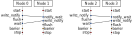
\includegraphics[width=\textwidth]{img/bench-ping-pong}
\caption{Visualization of the data transfer in the ping pong benchmark.}
\label{img:impl:ubench:ping-pong}
\end{figure}

\begin{table}[htb]
\centering
\begin{tabular}{c|ccccccc}
\bfseries Name & \bfseries Bytes & \tblcellsplit{\bfseries Repe- \\ \bfseries titions} & \tblcellsplit{\bfseries Time \\ \bfseries min.} & \tblcellsplit{\bfseries Time \\ \bfseries max.} & \tblcellsplit{\bfseries Time \\ \bfseries avg.} & \tblcellsplit{\bfseries Band- \\ \bfseries width} & \bfseries \tblcellsplit{Ops. \\ per sec.} \\\hline
\tblcellsplit{Ping- \\ Pong} & \yes & \yes & \yes& \yes & \yes & \yes & \no
\end{tabular}
\caption{Output report settings for the ping pong benchmark.}
\label{tbl:impl:ubench:ping-pong}
\end{table}

\subsection{Unidirectional Put}
\label{ssec:impl:ubench:put-udir}

The next series of benchmarks is used to investigate the fundamental communication primitives. First, the \emph{put} routine is evaluated. In this unidirectional put benchmark, communication is performed from one sender node to one receiver node. There exist two variations of this benchmark: The \emph{single unidirectional put} benchmark and the \emph{all unidirectional put} benchmark. Both benchmarks measure transfer bandwidth, hence the output statistics are collected as per \autoref{tbl:impl:ubench:put-udir}.


\begin{table}[htb]
\centering
\begin{tabular}{c|ccccccc}
\bfseries Name & \bfseries Bytes & \tblcellsplit{\bfseries Repe- \\ \bfseries titions} & \tblcellsplit{\bfseries Time \\ \bfseries min.} & \tblcellsplit{\bfseries Time \\ \bfseries max.} & \tblcellsplit{\bfseries Time \\ \bfseries avg.} & \tblcellsplit{\bfseries Band- \\ \bfseries width} & \bfseries \tblcellsplit{Ops. \\ per sec.} \\\hline
\tblcellsplit{Unidirectional \\ Put} & \yes & \yes & \yes& \yes & \yes & \yes & \no
\end{tabular}
\caption{Output report settings for both unidirectional put benchmarks.}
\label{tbl:impl:ubench:put-udir}
\end{table}

\subsubsection*{Single Unidirectional Put}
The \emph{single unidirectional put} benchmark operates on exactly two processes. All other additional ranks wait on a common barrier call. The data exchange is initiated by the first rank and targets the second rank. Along with the data, a notification is sent with the combined call \gaspiWriteNotify in order to provide accurate time measurement at the receiving end. 

The visualization is depicted in \autoref{img:impl:ubench:put-single-udir}. It can be observed that only the first two ranks are involved in the actual data exchange and that data is only transferred in one direction.

\begin{figure}[htb]
\centering
\includegraphics[width=0.8\textwidth]{img/bench-put-single-udir}
\caption{Visualization of the data transfer in the \emph{single unidirectional put} benchmark.}
\label{img:impl:ubench:put-single-udir}
\end{figure}

\subsubsection*{All Unidirectional Put}

A variation of the single unidirectional put benchmark is the \emph{all unidirectional put} scheme: Instead of only involving transfers from the first to the second node, the first node will now transmit data to every other node. The receiving nodes will wait for transmission to be completed by waiting for the notification sent in succession to each write operation. Since all \ac{RMA} operations target different ranks, no efficiency gain can be achieved by deferring notifications after all write operations have been scheduled.

In \autoref{img:impl:ubench:put-all-udir} the benchmark is visualized: All ranks are involved in the data exchange and receive data from the master node in a sequential fashion.


\begin{figure}[htb]
\centering
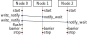
\includegraphics[width=0.8\textwidth]{img/bench-put-all-udir}
\caption{Visualization of the data transfer in the \emph{all unidirectional put} benchmark.}
\label{img:impl:ubench:put-all-udir}
\end{figure}

The output characteristics of the benchmark are shown in \autoref{tbl:impl:ubench:put-udir}. In contrast to the single unidirectional benchmark, more than one single block of data is transferred. The bandwidth obtained from dividing the transfer size by the full execution latency must therefore be multiplied with a factor that corresponds to the number of active nodes: If $n$ nodes are participating in the benchmark, $n-1$ blocks of data have been transferred. Therefore, the calculated bandwidth must be multiplied with $n-1$.


\subsection{Bidirectional Put}
\label{ssec:impl:ubench:put-bdir}

In order to measure concurrent access, the bidirectional put benchmarks exist. Comparable to the unidirectional put benchmarks, the bidirectional mode is divided into two parts: One for transfers between only two nodes and one benchmark for transfers among all nodes. The output report configuration is shown in \autoref{tbl:impl:ubench:put-bdir} for both benchmark variations. 

\begin{table}[htb]
\centering
\begin{tabular}{c|ccccccc}
\bfseries Name & \bfseries Bytes & \tblcellsplit{\bfseries Repe- \\ \bfseries titions} & \tblcellsplit{\bfseries Time \\ \bfseries min.} & \tblcellsplit{\bfseries Time \\ \bfseries max.} & \tblcellsplit{\bfseries Time \\ \bfseries avg.} & \tblcellsplit{\bfseries Band- \\ \bfseries width} & \bfseries \tblcellsplit{Ops. \\ per sec.} \\\hline
\tblcellsplit{Bidirectional \\ Put} & \yes & \yes & \yes& \yes & \yes & \yes & \no
\end{tabular}
\caption{Output report settings for both bidirectional put benchmarks.}
\label{tbl:impl:ubench:put-bdir}
\end{table}

\subsubsection*{Single Bidirectional Put}

The \emph{single bidirectional put} benchmark transfers data between exactly two nodes. Both transfers are executed in parallel, independent from each other. All other additional nodes wait on a common barrier call and are otherwise not involved in the transfer.

The illustration of the transmission scheme is depicted in \autoref{img:impl:ubench:put-single-bdir}. It can be observed that the transfer happens in a parallel fashion. Both nodes involved wait for the notification of the respective other node in order to mark the transmission as completed. Because of this parallelism, the reported bandwidth is not multiplied: It can be seen that two transfers happen in total but the reported bandwidth is regarded as a unidirectional metric. If the interconnection network is designed to support full duplex transmissions, a separated channel for receiving and transmitting data exists. Therefore the full bandwidth should be measurable even if data is transferred in both directions on a link. 

\begin{figure}[htb]
\centering
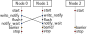
\includegraphics[width=0.8\textwidth]{img/bench-put-single-bdir}
\caption{Visualization of the data transfer in the \emph{single bidirectional put} benchmark.}
\label{img:impl:ubench:put-single-bdir}
\end{figure}

\subsubsection*{All Bidirectional Put}

The \emph{all bidirectional put} benchmark involves all ranks of the parallel program. During the benchmark each rank transfers a block of data to each other remote rank. Consequently, each rank also receives a block of data from each other remote rank. In order to avoid congestion, the transfers are queued in a modulo fashion, so that in one time step all transfers target different nodes. The \ac{GASPI} standard guarantees no ordering so that this benchmark may also be used to check if the \ac{GASPI} implementation schedules transfers in a advantageous way or if manual intervention is required. This intervention may be in the form of a flush operation after scheduling the \ac{RMA} operation to a node in order to ensure that the transfer has been executed.

The transfer scheme is depicted in \autoref{img:impl:ubench:put-all-bdir}. To provide a more comprehensible visualization, the communication partners are displayed as text on the arrows. It can easily be seen that all nodes execute the exact same operations and that only the target nodes vary. It shall be mentioned that the order of reception for the notifications may not be predicted. The order displayed in \autoref{img:impl:ubench:put-all-bdir} is sensible, since the transfers are executed in that order. The \ac{GASPI} standard, however, does not include ordering rules for transfers to different ranks.


\begin{figure}[htb]
\centering
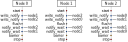
\includegraphics[width=\textwidth]{img/bench-put-all-bdir}
\caption{Visualization of the data transfer in the \emph{all bidirectional put} benchmark.}
\label{img:impl:ubench:put-all-bdir}
\end{figure}


For calculating the achieved bandwidth the quotient of transfer size and execution latency is multiplied with $n-1$, with $n$ as the number of ranks in the \ac{GASPI} environment. This is because one node sends data to all other nodes but to itself. The total number of transmissions is larger, since one node also receives data from other nodes. Regarding the bandwidth calculation the same argument presented along with the single bidirectional put benchmark applies: In full duplex systems, the concurrent reception of data should be non-interfering with a send operation. Furthermore, due to the modulo transmission order, the write operations targeting different nodes should also not interfere with each other. From \autoref{img:impl:ubench:put-all-bdir} it can be seen that in each \enquote{time step} each node transmits data to a different node, therefore providing a maximum degree of efficiency.

\subsection{Unidirectional Get}
\label{ssec:impl:ubench:get-udir}

The benchmarks for the \emph{get} primitives are structured in the same way as the \emph{put} benchmarks: They are differentiated in unidirectional and bidirectional as well as single versus global communication. In contrast to the put benchmarks, the notifications are now delivered to the initiating node. The remote node is not involved in the transfers at all. Comparable to the put benchmarks, the unidirectional get benchmarks also report execution latency and achieved bandwidth as per \autoref{tbl:impl:ubench:get-udir}.

\begin{table}[htb]
\centering
\begin{tabular}{c|ccccccc}
\bfseries Name & \bfseries Bytes & \tblcellsplit{\bfseries Repe- \\ \bfseries titions} & \tblcellsplit{\bfseries Time \\ \bfseries min.} & \tblcellsplit{\bfseries Time \\ \bfseries max.} & \tblcellsplit{\bfseries Time \\ \bfseries avg.} & \tblcellsplit{\bfseries Band- \\ \bfseries width} & \bfseries \tblcellsplit{Ops. \\ per sec.} \\\hline
\tblcellsplit{Unidirectional \\ Get} & \yes & \yes & \yes& \yes & \yes & \yes & \no
\end{tabular}
\caption{Output report settings for both bidirectional put benchmarks.}
\label{tbl:impl:ubench:get-udir}
\end{table}

\subsubsection*{Single Unidirectional Get}

The \emph{single unidirectional get} benchmark involves the first two ranks in the communication. Only the first rank executes different code than all other ranks, since the get routine implements a true one-sided scheme. In an application benchmark, a notification would be required prior to issuing the get operation to inform the initiating node that valid data is available.

In \autoref{img:impl:ubench:get-single-udir} the transmission scheme is depicted. The arrows next to the respective operation indicate the target rank. It can clearly be seen that only one node is actively involved in the transfer. Only one single transfer is performed, therefore the measured quotient of transfer size and execution latency is not multiplied with any correctional factor.

\begin{figure}[htb]
\centering
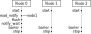
\includegraphics[width=0.8\textwidth]{img/bench-get-single-udir}
\caption{Visualization of the data transfer in the \emph{single unidirectional get} benchmark.}
\label{img:impl:ubench:get-single-udir}
\end{figure}

\subsubsection*{All Unidirectional Get}

The \emph{all unidirectional get} benchmark passively involves all ranks. The first rank is actively involved in the communication pattern and executes a series of read operations to fetch data from all other nodes. Consecutively, the first rank waits for the data to arrive. All other nodes wait on a common barrier and take no part in the program code of the communication.

The visualization is shown in \autoref{img:impl:ubench:get-all-udir}. Since the number of nodes may potentially be large, the algorithm takes care of selecting a \ac{GASPI} queue that still has sufficient capacity. During the flush operation all queues that have been used are flushed.

\begin{figure}[htb]
\centering
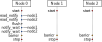
\includegraphics[width=0.9\textwidth]{img/bench-get-all-udir}
\caption{Visualization of the data transfer in the \emph{all unidirectional get} benchmark.}
\label{img:impl:ubench:get-all-udir}
\end{figure}

To calculate the bandwidth, the quotient of transfer size and execution latency is multiplied with $n-1$ with $n$ corresponding to the number of active \ac{GASPI} ranks. This is correct, since $n-1$ blocks of data have been fetched over the same transmission channel.

\subsection{Bidirectional Get}

The final set of get benchmarks concerns bidirectional transfers using the \emph{get} primitive. Comparable to the bidirectional put benchmarks in \secref{ssec:impl:ubench:put-bdir}, multiple nodes are now involved in the issuing of \ac{RMA} operations. This set of benchmarks measures the achieved bandwidth as its most important characteristic. Therefore, the output metrics reported by this benchmark consist of the execution time and the calculated bandwidth again. The list of metrics can be identified in \autoref{tbl:impl:ubench:get-bdir}.

\begin{table}[htb]
\centering
\begin{tabular}{c|ccccccc}
\bfseries Name & \bfseries Bytes & \tblcellsplit{\bfseries Repe- \\ \bfseries titions} & \tblcellsplit{\bfseries Time \\ \bfseries min.} & \tblcellsplit{\bfseries Time \\ \bfseries max.} & \tblcellsplit{\bfseries Time \\ \bfseries avg.} & \tblcellsplit{\bfseries Band- \\ \bfseries width} & \bfseries \tblcellsplit{Ops. \\ per sec.} \\\hline
\tblcellsplit{Bidirectional \\ Get} & \yes & \yes & \yes& \yes & \yes & \yes & \no
\end{tabular}
\caption{Output report settings for both bidirectional get benchmarks.}
\label{tbl:impl:ubench:get-bdir}
\end{table}


\subsubsection*{Single Bidirectional Get}

In the \emph{single bidirectional get} benchmark two blocks of data are exchanged from different nodes. Only the first two nodes are actively involved in the transfer. All other nodes wait on a collective barrier call. The transfer is executed in a concurrent way: While the first node fetches the block of data from the second rank, data is also fetched from the first rank by the second rank.

The scheme is visualized in \autoref{img:impl:ubench:get-single-bdir}. It can be seen that the first two ranks execute identical program code except for the specification of the target rank. All other nodes are not involved in any operation, actively or passively.

\begin{figure}[htb]
\centering
\includegraphics[width=0.9\textwidth]{img/bench-get-single-bdir}
\caption{Visualization of the data transfer in the \emph{single bidirectional get} benchmark.}
\label{img:impl:ubench:get-single-bdir}
\end{figure}

The measured bandwidth is not multiplied with a correctional factor since the transfer happens in a parallel fashion: From the perspective of one node one block of data is transmitted while simultaneously another block is received.


\subsubsection*{All Bidirectional Get}

Last, the \emph{all bidirectional get} benchmark complete the series of the fundamental transfer benchmarks. In this benchmark all nodes are actively involved in the transfer and fetch a block of data from each other node. After receiving the notifications that all \ac{RMA} operations are concluded a global barrier is invoked to synchronize all ranks. 

The transfer scheme is depicted in \autoref{img:impl:ubench:get-all-bdir}. It is noticeable that all ranks execute the exact same program code, except for the selection of the respective target nodes. In order to avoid congestion when concurrently fetching data with all nodes, the target ranks are selected in a modulo fashion, like in the bidirectional put benchmarks presented in \secref{ssec:impl:ubench:put-bdir}

\begin{figure}[htb]
\centering
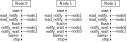
\includegraphics[width=0.9\textwidth]{img/bench-get-all-bdir}
\caption{Visualization of the data transfer in the \emph{all bidirectional get} benchmark.}
\label{img:impl:ubench:get-all-bdir}
\end{figure}

The obtained bandwidth is multiplied with a factor of $n-1$ with $n$ as the number of total \ac{GASPI} ranks. This is correct, since the number of transfers in one direction on one single nodes equals $n-1$. In total, $n\cdot (n-1)$ transfers are executed during the benchmark in the system -- $n$ of these are executed in parallel  in one \enquote{time step}.


\subsection{Allreduce Collective}

The allreduce collective benchmark seeks to evaluate the \gaspiAllreduce function. The functionality of the \gaspiAllreduce routine is explained in \secref{ssec:background:gaspi:collective-atomic}. Collective operations  that involve a group must be executed by all ranks of the group. Since the \gaspiAllreduce can be configured to use \code{GASPI\_BLOCK} as the timeout setting, a blocking behavior of the function is realized that is advantageous for measurement in a benchmark.

In the benchmark's implementation, the reduction is performed using \code{int} types. The \ac{GASPI} standard supports a variety of different types such as \code{double}, \code{uint} or \code{long}. The \code{int} type has the smallest bit-length of the available types \cite[ch.~11.3.3]{gaspi-std}.

As explained in \secref{ssec:background:gaspi:collective-atomic}, three different predefined reduction operators exist. The benchmark is written in a generic way so that it may be run with different reduction operators. The evaluation of all three operators for determining the minimum, the maximum and the sum of the data set is part of the benchmarking suite.

Since the actual amount of exchanged data is neither visible to the user nor defined by the \ac{GASPI} standard, providing a measurement result in terms of bandwidth is not possible. Instead, the operation rate may be reported. The data size included in the benchmark report is related to the number of elements processed by \gaspiAllreduce and therefore is a multiple of \code{sizeof(int)}. The full list of output metrics is given in \autoref{tbl:impl:ubench:allreduce}.

\begin{table}[htb]
\centering
\begin{tabular}{c|ccccccc}
\bfseries Name & \bfseries Bytes & \tblcellsplit{\bfseries Repe- \\ \bfseries titions} &\tblcellsplit{\bfseries Time \\ \bfseries min.} & \tblcellsplit{\bfseries Time \\ \bfseries max.} & \tblcellsplit{\bfseries Time \\ \bfseries avg.} & \tblcellsplit{\bfseries Band- \\ \bfseries width} & \bfseries \tblcellsplit{Ops. \\ per sec.} \\\hline
Allreduce & \yes & \yes & \yes & \yes & \yes & \no & \yes
\end{tabular}
\caption{Output report settings for the allreduce benchmarks.}
\label{tbl:impl:ubench:allreduce}
\end{table}

\subsection{Barrier Collective}
\label{ssec:impl:barrier}

The most simple benchmark is the measurement of the barrier collective operation. Its purpose is to evaluate the latency of a global barrier call. In the benchmark all nodes start the time measurement, perform one collective barrier and then stop the measurement. 

Since the benchmark does not depend on a transfer size, it is not repeated for a varying number of bytes like the other benchmarks previously presented. The central metric that is measured is the number of operations per second. The full list of metrics gathered is shown in \autoref{tbl:impl:ubench:barrier}.

\begin{table}[htb]
\centering
\begin{tabular}{c|ccccccc}
\bfseries Name & \bfseries Bytes & \tblcellsplit{\bfseries Repe- \\ \bfseries titions} &\tblcellsplit{\bfseries Time \\ \bfseries min.} & \tblcellsplit{\bfseries Time \\ \bfseries max.} & \tblcellsplit{\bfseries Time \\ \bfseries avg.} & \tblcellsplit{\bfseries Band- \\ \bfseries width} & \bfseries \tblcellsplit{Ops. \\ per sec.} \\\hline
Barrier & \no & \yes & \yes & \yes & \yes & \no & \yes
\end{tabular}
\caption{Output report settings for the barrier benchmark.}
\label{tbl:impl:ubench:barrier}
\end{table}


\subsection{Atomics}

A selection of benchmarks for atomic operations from the \ac{GASPI} library is implemented. As presented in \secref{ssec:background:gaspi:collective-atomic}, the two defined atomic operations are \emph{fetch and add} and \emph{compare and swap}. Again, there exist two variations of the benchmark for each atomic operation: A \emph{single} and one \emph{all} version. Like the barrier collective benchmark, atomic operations do not rely on a transfer size. Hence, the central figure for performance is the number of operations per second. All other generated benchmark result metrics are shown in \autoref{tbl:impl:ubench:atomic}.

\begin{table}[htb]
\centering
\begin{tabular}{c|ccccccc}
\bfseries Name & \bfseries Bytes & \tblcellsplit{\bfseries Repe- \\ \bfseries titions} &\tblcellsplit{\bfseries Time \\ \bfseries min.} & \tblcellsplit{\bfseries Time \\ \bfseries max.} & \tblcellsplit{\bfseries Time \\ \bfseries avg.} & \tblcellsplit{\bfseries Band- \\ \bfseries width} & \bfseries \tblcellsplit{Ops. \\ per sec.} \\\hline
Atomic & \no & \yes & \yes & \yes & \yes & \no & \yes
\end{tabular}
\caption{Output report settings for the atomic benchmarks.}
\label{tbl:impl:ubench:atomic}
\end{table}

\subsubsection*{Single Fetch and Add}

The \emph{single fetch and add} benchmark is comparable to the \emph{fetch and add} benchmark of the \ac{IMB} suite: Only the first rank executes a single \emph{fetch and add} operation while all other ranks wait on a common barrier call. The \emph{fetch and add} operation targets the second rank and atomically updates one value in a shared memory segment. A visualization is provided in \autoref{img:impl:ubench:faa-single}.

\begin{figure}[htb]
\centering
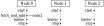
\includegraphics[width=0.9\textwidth]{img/bench-atomic-faa-single}
\caption{Visualization of the operation in the \emph{single fetch and add} benchmark.}
\label{img:impl:ubench:faa-single}
\end{figure}

\subsubsection*{All Fetch and Add}

A variation of the \emph{single fetch and add} benchmark is implemented in the \emph{all fetch and add} benchmark. In this scheme all nodes except the first try to update a value located on the first node. The objective of the benchmark is to measure the effects of concurrent parallel access from all nodes to one single node. The implementation of the \emph{fetch and add} routine must ensure consistency so that parallel update requests are partially serialized  in order to guarantee reproducible correct results. The scheme is shown in \autoref{img:impl:ubench:faa-all}. In comparison to \autoref{img:impl:ubench:faa-single} the first rank is only passively involved in the process, since it serves as the target for the \emph{fetch and add} operation.

\begin{figure}[htb]
\centering
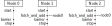
\includegraphics[width=0.9\textwidth]{img/bench-atomic-faa-all}
\caption{Visualization of the operation in the \emph{all fetch and add} benchmark.}
\label{img:impl:ubench:faa-all}
\end{figure}

\subsubsection*{Single Compare and Swap}

The second atomic operation in addition to \emph{fetch and add} is \emph{compare and swap}. This operation atomically changes a value in a remote memory location if the current value is equal to a given other value. Since the function's signature is comparable to the \emph{fetch and add} operation, the benchmarks are structured similarly. In the first \emph{compare and swap} benchmark, only the first two ranks are involved in the atomic operation: The first rank attempts to compare and swap a value on a remote memory segment on the second rank. All other ranks wait on a common barrier call. The scheme is visualized in \autoref{img:impl:ubench:cas-single}. 

\begin{figure}[htb]
\centering
\includegraphics[width=\textwidth]{img/bench-atomic-cas-single}
\caption{Visualization of the operation in the \emph{single compare and swap} benchmark.}
\label{img:impl:ubench:cas-single}
\end{figure}


\subsubsection*{All Compare and Swap}

Comparable to the \emph{all fetch and add} benchmark, a similar \emph{all compare and swap} benchmark exists. All \ac{GASPI} ranks except for the first rank try to concurrently access the same remote memory value located at the first rank. Since the operation is atomic, only one of the other ranks will successfully swap the value while the compare step will prevent all other nodes from modifying the remote value. The procedure is depicted in \autoref{img:impl:ubench:cas-all}.

\begin{figure}[htb]
\centering
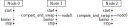
\includegraphics[width=\textwidth]{img/bench-atomic-cas-all}
\caption{Visualization of the operation in the \emph{all compare and swap} benchmark.}
\label{img:impl:ubench:cas-all}
\end{figure}


\subsection{Notification Rate}

In the fundamental put and get benchmarks, all \ac{RMA} operations were succeeded by a notification to indicate the successful conclusion of the operation. In this benchmark, the raw notification rate is measured: Notifications are sent to another node and consumed on the remote side. To conform with the other benchmarks presented in this chapter, the notification microbenchmarks are subdivided into four benchmarks to evaluate the combinations of single versus all and unidirectional versus bidirectional notifications. Since a notification does not transport any payload data, this benchmark does not depend on a transmission size and therefore does not report an achieved bandwidth. The measured metrics are shown in \autoref{tbl:impl:ubench:notification}.

\begin{table}[htb]
\centering
\begin{tabular}{c|ccccccc}
\bfseries Name & \bfseries Bytes & \tblcellsplit{\bfseries Repe- \\ \bfseries titions} &\tblcellsplit{\bfseries Time \\ \bfseries min.} & \tblcellsplit{\bfseries Time \\ \bfseries max.} & \tblcellsplit{\bfseries Time \\ \bfseries avg.} & \tblcellsplit{\bfseries Band- \\ \bfseries width} & \bfseries \tblcellsplit{Ops. \\ per sec.} \\\hline
Notification & \no & \yes & \yes & \yes & \yes & \no & \yes
\end{tabular}
\caption{Output report settings for the notification benchmarks.}
\label{tbl:impl:ubench:notification}
\end{table}

\subsubsection*{Single Unidirectional Notification}

In the single unidirectional notification benchmark the first ranks sends a notification to the second rank. The second rank awaits the notification. All other ranks are not involved in the procedure and wait on a common barrier. After the notification is sent on the first rank, the single used \ac{GASPI} queue is flushed. The scheme is depicted in \autoref{img:impl:ubench:noti-single-udir}.

\begin{figure}[htb]
\centering
\includegraphics[width=\textwidth]{img/bench-noti-single-udir}
\caption{Visualization of the single unidirectional notification benchmark.}
\label{img:impl:ubench:noti-single-udir}
\end{figure}


\subsubsection*{All Unidirectional Notification}

Comparable to the \ac{RMA} benchmarks, the all unidirectional notification benchmark measures the latency of sending one notification to every rank, except for the first. The first rank sends the notifications to all other ranks in ascending order. After issuing all notification transmissions, potentially several used \ac{GASPI} queues are flushed. All other nodes wait for one single notification issued by the first rank. The process is visualized in \autoref{img:impl:ubench:noti-all-udir}.

\begin{figure}[htb]
\centering
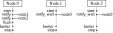
\includegraphics[width=\textwidth]{img/bench-noti-all-udir}
\caption{Visualization of the all unidirectional notification benchmark.}
\label{img:impl:ubench:noti-all-udir}
\end{figure}


\subsubsection*{Single Bidirectional Notification}

In the single bidirectional notification benchmark one notification is sent and received from and by the first two ranks: The first rank sends a notification to the seconds rank and vice versa. Both transmissions are executed in parallel. All other nodes wait on a common barrier call and are not involved in the communication scheme that is visualized in \autoref{img:impl:ubench:noti-single-bdir}.

\begin{figure}[htb]
\centering
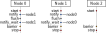
\includegraphics[width=\textwidth]{img/bench-noti-single-bdir}
\caption{Visualization of the single bidirectional notification benchmark.}
\label{img:impl:ubench:noti-single-bdir}
\end{figure}

\subsubsection*{All Bidirectional Notification}

Finally, in the all bidirectional notification benchmark, every node sends and receives an equal amount of notifications. The number of notifications sent and received from and by each node is $n-1$ with $n$ as the number of active \ac{GASPI} ranks. After all notifications are sent, the  \ac{GASPI} queues used in the process are flushed and the ranks wait for the $n-1$ notifications to arrive. In order to prevent the notifications from overwriting each other at one node, notifications are tagged with the number of the sending rank. The scheme is displayed in \autoref{img:impl:ubench:noti-all-bdir}.

\begin{figure}[htb]
\centering
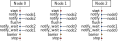
\includegraphics[width=\textwidth]{img/bench-noti-all-bdir}
\caption{Visualization of the all bidirectional notification benchmark.}
\label{img:impl:ubench:noti-all-bdir}
\end{figure}

\subsection{True One-Sided Exchange}

The true one-sided communication benchmark is adapted from the \code{Truly\_\allowbreak pas\-sive\_\allowbreak put} benchmark of the \ac{IMB} \ac{RMA} benchmarking suite. Its objective is to determine if a one-sided \ac{RMA} operation really only involves the initiating side and does not affect the application. In prior benchmarks, the remote side was either waiting in a barrier call or on the arrival of a notification. Both operations are part of the \ac{GASPI} stack. In this benchmark the transmission latency between the first two ranks is first measured by executing either the single unidirectional put or get benchmark described in \secref{ssec:impl:ubench:put-udir} and \secref{ssec:impl:ubench:get-udir}. After this time has been determined, the remote side performs artificial computationally intensive workload for the measured time. The workload is generated by repeated multiplication of sufficiently large matrices. Concurrently to the workload on the remote side, the first rank attempts to transfer a memory block to or from the remote side with the put or get routine. 

By generating workload outside the \ac{GASPI} framework it can be measured if the \ac{RMA} routine can make progress on the remote side. If the \ac{GASPI} implementation or the underlying hardware does not support concurrent processing, the measured bandwidth will be much lower than the one measured in the single unidirectional put or get benchmark. These benchmarks are bandwidth-related, hence the output reports in \autoref{tbl:impl:ubench:true-onsided} are comparable to the put or get benchmarks.
 

\begin{table}[htb]
\centering
\setlength{\tabcolsep}{0.49em}
\begin{tabular}{c|ccccccc}
\bfseries Name & \bfseries Bytes & \tblcellsplit{\bfseries Repe- \\ \bfseries titions} &\tblcellsplit{\bfseries Time \\ \bfseries min.} & \tblcellsplit{\bfseries Time \\ \bfseries max.} & \tblcellsplit{\bfseries Time \\ \bfseries avg.} & \tblcellsplit{\bfseries Band- \\ \bfseries width} & \bfseries \tblcellsplit{Ops. \\ per sec.} \\\hline
\tblcellsplit{True one- \\ sided exchange}  & \yes & \yes & \yes & \yes & \yes & \yes & \no
\end{tabular}
\caption{Output report settings for the true one-sided exchange benchmarks.}
\label{tbl:impl:ubench:true-onsided}
\end{table}


\subsubsection*{Put Benchmark}

In the true one-sided put benchmark, the data is transferred using the put \ac{RMA} operation. To acquire the transmission latency, the previously presented single unidirectional put benchmark from \secref{ssec:impl:ubench:put-udir} is executed. After this, the first rank attempts to transmit another block of data to the second rank while the second rank executes unrelated computations for the previously determined transmission latency. The first rank sends a completion notification along with the data block that is processed by the second rank as soon as the unrelated computation has concluded. The full transmission scheme is depicted in \autoref{img:impl:ubench:true-onsided-put}. Comparable to the single unidirectional put benchmark, all other nodes are not involved in the transmission scheme.

\begin{figure}[htb]
\centering
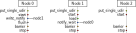
\includegraphics[width=\textwidth]{img/bench-true-one-sided-put}
\caption{Visualization of true one-sided put benchmark.}
\label{img:impl:ubench:true-onsided-put}
\end{figure}


\subsubsection*{Get Benchmark}

The true one-sided get benchmark uses the \ac{RMA} routine \emph{get} to transfer the data. First, the transfer latency is obtained by executing the single unidirectional get benchmark, discussed in \secref{ssec:impl:ubench:get-udir}. Afterwards, the first rank reads a block of remote memory from the second rank while the second rank performs unrelated computations for the time of the transfer latency. After the block has been successfully copied to the first rank, the completion notification is received. Other nodes apart from the first two are not involved in the measurement. The entire transmission scheme is shown in \autoref{img:impl:ubench:true-onsided-get}.

\begin{figure}[htb]
\centering
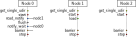
\includegraphics[width=\textwidth]{img/bench-true-one-sided-get}
\caption{Visualization of the true one-sided get benchmark.}
\label{img:impl:ubench:true-onsided-get}
\end{figure}


\subsection{Two-Sided Ping Pong}
\label{ssec:impl:ubench:two-sided}

Last, the two-sided communication routines described in \secref{ssec:background:gaspi:two-sided} are evaluated.  This is done with a simple ping pong benchmark. The transmission scheme is analogous to the \ac{RMA} ping pong benchmark shown in \secref{ssec:impl:ubench:ping-pong}. The visualization of the benchmark is shown in \autoref{img:impl:ubench:two-sided}. It can be observed that in comparison to \autoref{img:impl:ubench:ping-pong} no wait statements are necessary since the \gaspiPassiveSend and \gaspiPassiveReceive functions are already blocking.

\begin{figure}[htb]
\centering
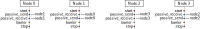
\includegraphics[width=\textwidth]{img/bench-twosided-ping-pong}
\caption{Visualization of the two-sided ping pong benchmark.}
\label{img:impl:ubench:two-sided}
\end{figure}

The benchmark is meant to measure the throughput of data, hence the achieved bandwidth is the key metric that is gained. Other generated information may be found in \autoref{tbl:impl:ubench:two-sided}. Since the transfer size is limited, the benchmark cannot be run for arbitrary transfer sizes. Through the benchmark initialization routines it is ensured that the requested transfer sizes conform to the maximal transfer sizes given by the \ac{GASPI} implementation.

\begin{table}[htb]
\centering
%\setlength{\tabcolsep}{0.49em}
\begin{tabular}{c|ccccccc}
\bfseries Name & \bfseries Bytes & \tblcellsplit{\bfseries Repe- \\ \bfseries titions} &\tblcellsplit{\bfseries Time \\ \bfseries min.} & \tblcellsplit{\bfseries Time \\ \bfseries max.} & \tblcellsplit{\bfseries Time \\ \bfseries avg.} & \tblcellsplit{\bfseries Band- \\ \bfseries width} & \bfseries \tblcellsplit{Ops. \\ per sec.} \\\hline
\tblcellsplit{Two-sided \\ ping pong}  & \yes & \yes & \yes & \yes & \yes & \yes & \no
\end{tabular}
\caption{Output report settings for the two-sided ping pong benchmarks.}
\label{tbl:impl:ubench:two-sided}
\end{table}


\section{Application Benchmarks}

Apart from the microbenchmarks, application benchmarks complement the benchmarking suite. These kind of benchmarks use communication schemes commonly found in real \ac{HPC} applications. Their purpose is to show the way of integrating new programming paradigms into real computational challenges and to evaluate the performance of programming models like \ac{GASPI} in an actual use case.



\subsection{Heat Expansion on a Grid with Halo Exchange}
\label{ssec:impl:grid}

The grid benchmark is a stencil application that computes the expansion of heat on a plane. The physical accuracy of the computation is of lesser importance -- the emphasis for the benchmark is put on the communication scheme. Fundamentally, the heat distribution is calculated in an iterative way. For each point in time a heat value for each of the point on a grid of defined size must be calculated. The calculation depends on prior heat values of that grid point as well as on prior values of points in the immediate vicinity of the target location. 

\subsubsection*{Calculation of an Iteration}

The grid on which the computation is performed is an arbitrary rectangular two-dimensional plane of a given resolution. To compute the temperature value for the next point in time, the current temperature value of the point and the values of the four neighboring points must be known. This is expressed in Equation \eqref{eq:impl:grid:formula} with $\text{T}_{r,c}^{'}$ as the new temperature value for the point in the row $r$ and the column $c$ and $\text{T}_{r,c}$ as the respective old temperature value. The coefficient $\Phi$ can be regarded as a \enquote{cooling} factor that causes the simulated heat to gradually decrease. An example grid with the visualization of the neighbors is shown in \autoref{img:impl:gridbench:grid-stencil}. It can be observed how the temperature values are shared among adjacent points to compute the new values for the point colored in red. Ultimately, all points of the grid must be updated to compute the result of one iteration.

\begin{equation}
\label{eq:impl:grid:formula}
\text{T}_{r,c}^{'} = (1 - 4 \cdot \Phi) \cdot \text{T}_{r,c} + \Phi \cdot (\text{T}_{r-1,c} + \text{T}_{r+1,c} + \text{T}_{r,c - 1} + \text{T}_{r,c + 1} );\quad \Phi=\frac{6}{25}.
\end{equation}

\begin{figure}[htb]
\centering
\includegraphics[width=0.8\textwidth]{img/bench-grid-stencil}
\caption{Grid layout and stencil computation scheme.}
\label{img:impl:gridbench:grid-stencil}
\end{figure}

\subsubsection*{Parallel Decomposition}

The previously presented iteration formula from Equation \eqref{eq:impl:grid:formula} can easily be implemented in a sequential program that uses two nested loops to iterate over all points on the grid. Special care must only be applied to the border regions where the number of neighbors is less than in the inner grid. For this benchmark it is defined that all points that exceed the grid have a temperature of zero. To compute the application on a distributed parallel system, the computation must be segmented. 

Each node calculates a segment of the full grid. This segment is called a \emph{shard}. Every shard consists of a number of rows from the original grid. Every row has the full length to minimize the overlapping region with the shards of other ranks. From the stencil scheme of \autoref{img:impl:gridbench:grid-stencil} it is evident that the inner points of a shard can be updated in a trivial fashion by iterating over all inner points of the shard. For the points that make up the first and last row of a shard, special treatment is required since their values depend on data from other shards.

In \autoref{img:impl:gridbench:grid-stencil-sharded} the distribution of the grid into shards is shown. The colored regions in blue and yellow are the data that is stored in the individual nodes. Each shard also includes a row at the top and at the bottom that overlaps with the adjacent shards' data. To make the algorithm less complicated, the border rows and columns of the full grid are also stored, even though they are defined to be zero. This allows for easy memory access. Consequently, the grid or shard which is actually stored in memory has two additional columns. For the treatment of the top and bottom border region the top shard contains one additional row and the bottom shard also contains an additional row. 

\begin{figure}[htb]
\centering

\includegraphics[width=0.9\textwidth]{img/bench-grid-stencil-sharded}
\caption{Stencil computation in a layout with shards.}
\label{img:impl:gridbench:grid-stencil-sharded}
\end{figure}

\subsubsection*{Communication Pattern}

After decomposing the grid into shards that are computed in parallel on different nodes, communication among the nodes is required to exchange the data in the overlapping region. This so called \emph{halo region} needs to be updated after each iteration on the full grid. If a consistent initial state is assumed, the application must perform the following steps:
\begin{enumerate}
	\item Calculate the grid increment of all points in the shard.
	\item Send top row to the shard above.
	\item Send bottom row to the shard below.
	\item Wait for the two adjacent shards until they send their halo data.
	\item Synchronize over all ranks.
	\item Calculate the next iteration.
\end{enumerate} 

The entire computation requires two shard buffers on each node: The first buffer contains the current state and the second buffer is used to gradually calculate the next state. Since the first buffer is only read from and the second buffer is only written to, this buffer concept may be easily adapted to \ac{RMA} operations. As soon as one rank finishes the first step from the list, it transmits the calculated data from the halo region into the active write buffer of the adjacent node. It may happen that the other node is also concurrently writing to this buffer but it is guaranteed that the memory locations are distinct and that no data is read from the write buffer. Therefore, race conditions with respect to data transfer concurrent to the computations can be avoided.

Since only the data-generating node has information whether its has computed all points, the data transmission is realized with the \gaspiWriteNotify routine. In comparison to two-sided \ac{MPI}-1 programs, the data transfer may overlap with computations or other work on the remote node since a posted receive operation is not required for \ac{RMA} operations. Since the data must be available prior to starting a new iteration, all nodes must wait for the notifications that the halo region has been updated by the adjacent ranks. After the data exchange is finished, the two shard buffers are switched on each node. This operation must be followed by a barrier, since this step affects the addressing of remote ranks. 

\subsubsection*{Multithreading}

Apart from the decomposition of the grid into shards the shards may be further broken down for the processing with multiple threads. Since threads share a common address space, a parallel processing of the shard involves only little additional modifications because explicit halo data exchange may be omitted.

The decomposition of the computation for threads is done similarly to the shard decomposition: When the shard is initialized, the rows of the shards are mapped to specific worker threads before the threads are launched. The computation is distributed as evenly as possible. This means that the amount of rows that one thread processes differ by one at most.

Since the \ac{GASPI} communication library is thread-safe for most routines, it is allowed for a \ac{GASPI} program to issue library calls from different threads. When the computation is done with multiple threads, only the threads that work on the rows in the halo region are involved in the data exchange. Since common data structures exist that are shared among all thread, they need to be secured for memory consistency. These shared data types especially include the two shard buffers. Modifications to this structure is guaranteed to be exclusive by a manually managed mutex variable. The buffers are switched by the last thread to finish an iteration -- all other threads are waiting on an event that is raised once the last thread has switched the buffers. 

The thread-based implementation is done with pthreads to allow for maximal flexibility in the design. Mutex and condition variables are taken from the pthread-library. 

\subsubsection*{Output Generation}

The benchmark is not bandwidth-orientated, since computation and communication overlaps. The central metric that may be gathered is the execution latency per iteration. This metric is coupled with the grid size because a larger grid requires more computations and hence more time per iteration. Each measurement is repeated multiple times to average fluctuations. Additionally, a series of warm-up repetitions are performed that are not reflected in the results reported. The following list of metrics is collected:

\begin{itemize}
	\item Grid size
	\item Number of repetitions
	\item Number of iterations on one grid
	\item Minimum time per iteration in microseconds
	\item Maximum time per iteration in microseconds
	\item Average time per iteration in microseconds
\end{itemize}

For debugging purposes and for proof of correctness the data of all shards may be collected and printed out. With the function \code{aggregateShardsRank0} all shards are aggregated at the first rank by using \ac{RMA} read operations. The resulting full grid may then be visualized -- for example in 3D with OpenGL, as shown in \autoref{img:impl:gridbench:grid-vis1}.

\begin{figure}[htb]
\centering
\includegraphics[width=0.6\textwidth]{img/gridbench-vis1}
\caption{3D visualization of the heat distribution rendered with OpenGL from the computed data.}
\label{img:impl:gridbench:grid-vis1}
\end{figure}

\section{Program Output Conversion}
\label{sec:impl:output-conversion}

In order to further process the benchmark results, an additional program has been developed. This utility program converts the output of the \ac{GBS} program into several \code{.csv} files -- one per benchmark. It was decided not to integrate the \acs{CSV}-compatible output generation into the \ac{GBS} suite because the \ac{IMB} and \ac{OMB} suites do not produce \acs{CSV}-compatible results either. Therefore, it is more straightforward to implement an external program that can process the output of the \ac{IMB}, \ac{OMB} and \ac{GBS} programs alike.  The developed application is written in plain ANSI-C without any additional requirements.

\subsection{General Features}

The application's fundamental purpose is to interpret the output of the \ac{IMB}, \ac{OMB} or \ac{GBS} program output and generate a \acs{CSV} file from them. \acs{CSV} files are useful if the data is to be processed in an automated fashion. Since the \ac{GBS} program output is fully compatible to the \ac{IMB} output, support must only be implemented for \ac{IMB} and \ac{OMB}. Special requirements for the format of the \ac{CSV} may exist, therefore the developed application features the following additional features:
\begin{itemize}
	\item Treatment of comments
	\begin{itemize}
		\item Replace the '\code{\#}' character that marks a comment in the \ac{IMB} or \ac{OMB} output with a different character.
		\item Strip all comments from the generated \acs{CSV} file.
	\end{itemize}
	\item Treatment of special characters (characters not in the range of A-Z, a-z or 0-9)
	\begin{itemize}
		\item Replace special characters with a common user-defined character.
		\item Strip all special characters from the generated \acs{CSV} file.
	\end{itemize}
	\item Definition of the \acs{CSV} separation character.
\end{itemize}

\subsection{Parsing of \acs{OMB} Files}

For the \ac{OMB} suite, separate programs exist for each benchmark. This means that only one benchmark may be generated at a time. When automating the benchmark execution it is most natural to redirect the output of the district benchmarks to different files -- hence, there exists one file with the results per benchmark. All benchmark data files have the structure depicted in \autoref{lst:impl:output-conversion:omb-raw}. The file can be segmented into a comment part, a header line and the data lines. The header line is the line that precedes the data. Everything above the header line is a comment. 

\begin{lstlisting}[style=console,captionpos={b},caption={Generated raw output of a \acs{OMB} run.},label=lst:impl:output-conversion:omb-raw]
# OSU MPI_Put Bandwidth Test v5.6.3
# Window creation: MPI_Win_allocate
# Synchronization: MPI_Win_flush
# Size      Bandwidth (MB/s)
1                       0.37
2                       0.74
4                       1.47
...
4194304               117.62
\end{lstlisting}

After the file has been processed, the output shown in \autoref{lst:impl:output-conversion:omb-csv} is generated. In the shown example all special characters have been removed and comment lines are introduced by the '\code{\%}' character.

\begin{lstlisting}[style=console,captionpos={b},caption={Processed \acs{OMB} output with replacement of the comment character with '\code{\%}' and removal of all special characters.},label=lst:impl:output-conversion:omb-csv]
% OSU MPI_Put Bandwidth Test v5.6.3
% Window creation: MPI_Win_allocate
% Synchronization: MPI_Win_flush
Size;BandwidthMBs
1;0.37
2;0.74
4;1.47
...
4194304;117.62
\end{lstlisting}



\subsection{Parsing of \acs{IMB} Files}

Output data generated from \ac{IMB} include more than one measurement. All benchmarks which were executed are concatenated in one single file. It is advantageous to split the results of the measurements into distinct \acs{CSV} files. In contrast to the \ac{OMB} processing, the \acs{CSV} files must be automatically named when processing the \ac{IMB} output. Therefore, the application is supplied with a directory name in which the generated output files are to be stored. The application chooses the \acs{CSV} file names according to the respective benchmark name which can be obtained from the \ac{IMB} output data. The structure of the data is comparable to the \ac{OMB} output and shown in \autoref{lst:impl:output-conversion:imb-raw}. It can be seen that the data for different benchmarks are directly concatenated. 

\begin{lstlisting}[style=console,captionpos={b},caption={Excerpt of the generated raw output of a \acs{IMB} run.},label=lst:impl:output-conversion:imb-raw]
#---------------------------------------------------
# Benchmarking PingPong
# #processes = 2
#---------------------------------------------------
       #bytes #repetitions      t[usec]   Mbytes/sec
            0         1000        25.75         0.00
            1         1000        26.34         0.04
          ...
      4194304           10     36087.92       116.22

#---------------------------------------------------
# Benchmarking PingPing
# #processes = 2
#---------------------------------------------------
       #bytes #repetitions      t[usec]   Mbytes/sec
            0         1000        49.05         0.00
            1         1000        49.00         0.02
            2         1000        49.25         0.04
          ...
\end{lstlisting}

After the data has been read in, the various benchmarks are separated and additional meta data in comments which is not shown in \autoref{lst:impl:output-conversion:imb-raw} is discarded. The benchmark data is processed in an identical fashion as the \ac{OMB} data. The final result of the application is a directory with \acs{CSV} files that contain the benchmark data, as shown in \autoref{lst:impl:output-conversion:imb-ls}.

\begin{lstlisting}[style=console,captionpos={b},caption={Listing of the result directory after processing an \ac{IMB} output file.},label=lst:impl:output-conversion:imb-ls]
user@machine: $ ls csv-directory
Allgather.csv Allreduce.csv Alltoallv.csv Bcast.csv Gather.csv PingPing.csv Reduce.csv Scatter.csv Sendrecv.csv Allgatherv.csv Alltoall.csv Barrier.csv Exchange.csv Gatherv.csv PingPong.csv Reduce_scatter.csv Scatterv.csv
\end{lstlisting}
